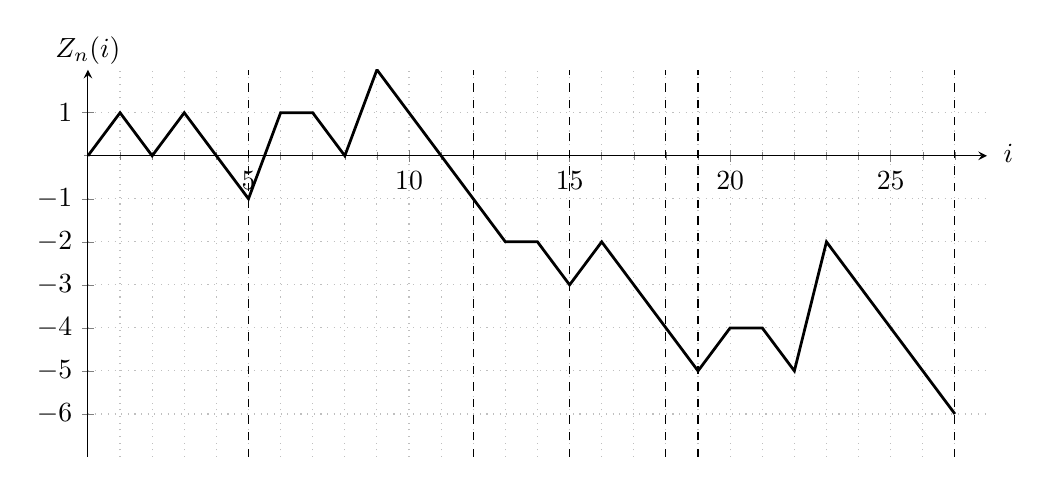
\begin{tikzpicture}

\begin{axis}[
axis x line=bottom,
axis y line=left,
grid = minor,
minor grid style={dotted},
xmin=0,
axis lines = middle,
xmax=28,
ymax = 2,
ymin  = -7,
xlabel={$i$},
x label style = {at={(axis description cs:1.04,0.785)},anchor=east},
ylabel={$Z_n(i)$},
y label style = {at={(axis description cs:0,1.11)},anchor=north},
xtick={5,10,15,20,25},
minor xtick = {1,...,27},
ytick={-6,...,1},
minor ytick={-6,...,1},
width = 13cm,
height = 6.5cm
]

\addplot [
line width=1.0pt
]
coordinates{
	(0,0) (1,1) (2,0) (3,1) (4,0) (5,-1)
	(6,1) (7,1) (8,0) (9,2) (10,1) (11,0) (12,-1) (13,-2) 
	(14,-2) (15,-3) 
	(16,-2) (17,-3) (18,-4) 
	(19,-5) 
	(20, -4) (21,-4) (22,-5) (23,-2) (24,-3) (25,-4) (26, -5) (27,-6)
};

\addplot [dashed] coordinates {(5, -7) (5, 2)};
\addplot [dashed] coordinates {(12, -7) (12, 2)};
\addplot [dashed] coordinates {(15, -7) (15, 2)};
\addplot [dashed] coordinates {(18, -7) (18, 2)};
\addplot [dashed] coordinates {(19, -7) (19, 2)};
\addplot [dashed] coordinates {(27, -7) (27, 2)};
\end{axis}

\end{tikzpicture} 